\documentclass[letterpaper,12pt]{article}\usepackage[]{graphicx}\usepackage[]{color}
%% maxwidth is the original width if it is less than linewidth
%% otherwise use linewidth (to make sure the graphics do not exceed the margin)
\makeatletter
\def\maxwidth{ %
  \ifdim\Gin@nat@width>\linewidth
    \linewidth
  \else
    \Gin@nat@width
  \fi
}
\makeatother

\definecolor{fgcolor}{rgb}{0.345, 0.345, 0.345}
\newcommand{\hlnum}[1]{\textcolor[rgb]{0.686,0.059,0.569}{#1}}%
\newcommand{\hlstr}[1]{\textcolor[rgb]{0.192,0.494,0.8}{#1}}%
\newcommand{\hlcom}[1]{\textcolor[rgb]{0.678,0.584,0.686}{\textit{#1}}}%
\newcommand{\hlopt}[1]{\textcolor[rgb]{0,0,0}{#1}}%
\newcommand{\hlstd}[1]{\textcolor[rgb]{0.345,0.345,0.345}{#1}}%
\newcommand{\hlkwa}[1]{\textcolor[rgb]{0.161,0.373,0.58}{\textbf{#1}}}%
\newcommand{\hlkwb}[1]{\textcolor[rgb]{0.69,0.353,0.396}{#1}}%
\newcommand{\hlkwc}[1]{\textcolor[rgb]{0.333,0.667,0.333}{#1}}%
\newcommand{\hlkwd}[1]{\textcolor[rgb]{0.737,0.353,0.396}{\textbf{#1}}}%
\let\hlipl\hlkwb

\usepackage{framed}
\makeatletter
\newenvironment{kframe}{%
 \def\at@end@of@kframe{}%
 \ifinner\ifhmode%
  \def\at@end@of@kframe{\end{minipage}}%
  \begin{minipage}{\columnwidth}%
 \fi\fi%
 \def\FrameCommand##1{\hskip\@totalleftmargin \hskip-\fboxsep
 \colorbox{shadecolor}{##1}\hskip-\fboxsep
     % There is no \\@totalrightmargin, so:
     \hskip-\linewidth \hskip-\@totalleftmargin \hskip\columnwidth}%
 \MakeFramed {\advance\hsize-\width
   \@totalleftmargin\z@ \linewidth\hsize
   \@setminipage}}%
 {\par\unskip\endMakeFramed%
 \at@end@of@kframe}
\makeatother

\definecolor{shadecolor}{rgb}{.97, .97, .97}
\definecolor{messagecolor}{rgb}{0, 0, 0}
\definecolor{warningcolor}{rgb}{1, 0, 1}
\definecolor{errorcolor}{rgb}{1, 0, 0}
\newenvironment{knitrout}{}{} % an empty environment to be redefined in TeX

\usepackage{alltt}
\usepackage[top=1in,bottom=1in,left=1in,right=1in]{geometry}
\usepackage{setspace}
\usepackage[colorlinks=true,urlcolor=blue,citecolor=blue,linkcolor=blue]{hyperref}
\usepackage{indentfirst}
\usepackage{multirow}
\usepackage{booktabs}
\usepackage[final]{animate}
\usepackage{graphicx}
\usepackage{verbatim}
\usepackage{rotating}
\usepackage{tabularx}
\usepackage{array}
\usepackage{subfig} 
\usepackage[noae]{Sweave}
\usepackage{cleveref}
\usepackage[figureposition=bottom]{caption}
\usepackage{paralist}
\usepackage{acronym}
\usepackage{outlines}
\usepackage{pdflscape}

% housekeeping


\linespread{1}
\IfFileExists{upquote.sty}{\usepackage{upquote}}{}
\begin{document}
\title{Analysis of crab abundance, presence/absence, and carapace length}
\maketitle



\begin{knitrout}
\definecolor{shadecolor}{rgb}{0.969, 0.969, 0.969}\color{fgcolor}
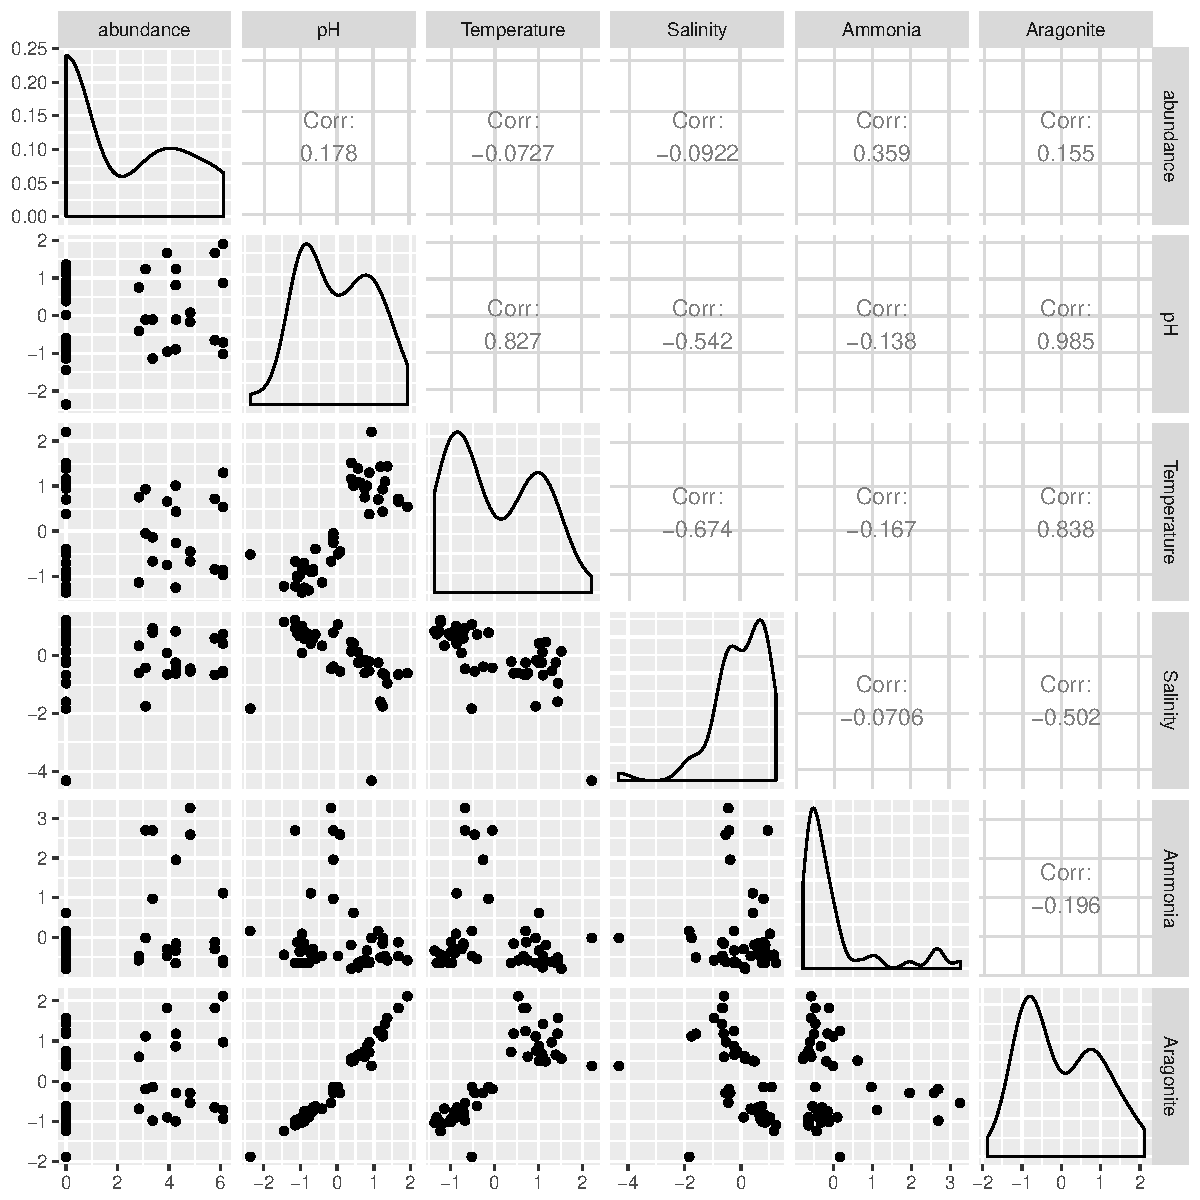
\includegraphics[width=\maxwidth]{figure/unnamed-chunk-3-1} 

\end{knitrout}



\begin{knitrout}
\definecolor{shadecolor}{rgb}{0.969, 0.969, 0.969}\color{fgcolor}\begin{figure}
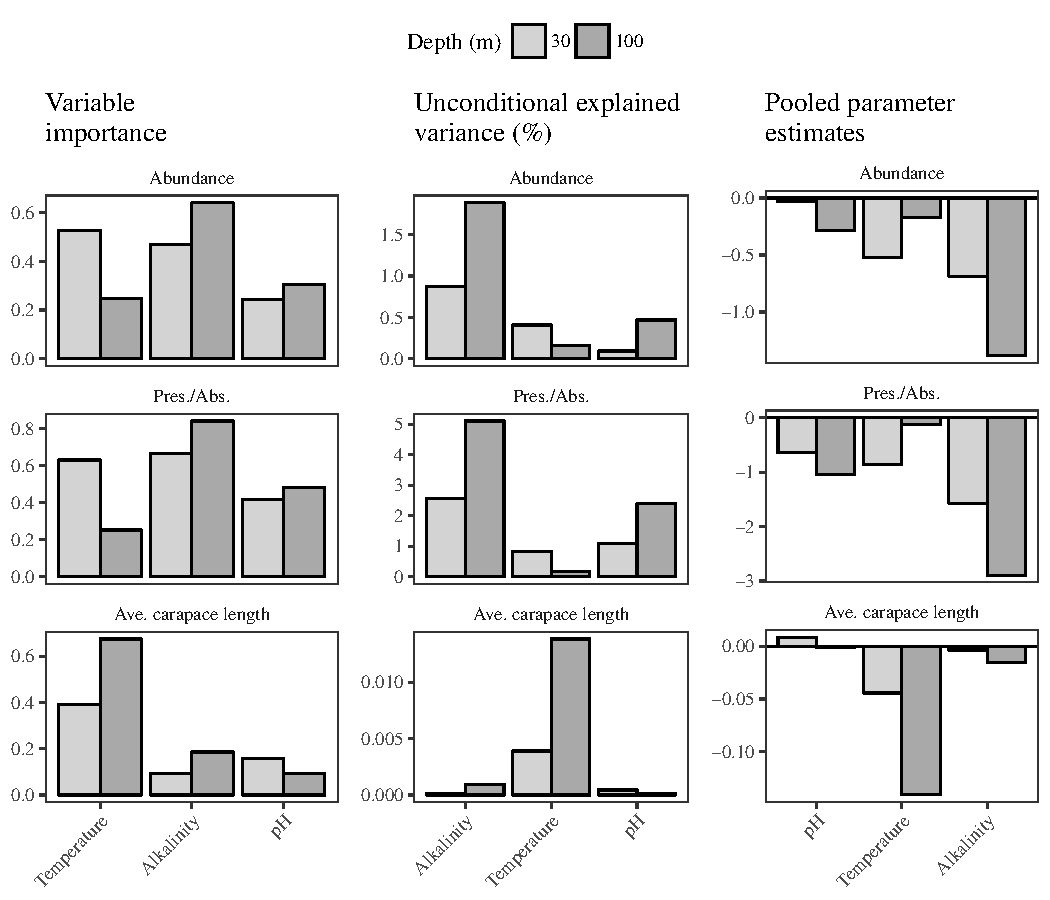
\includegraphics[width=\maxwidth]{figure/unnamed-chunk-5-1} \caption[Results of model selection analysis with three crab population variables (abundance, presence/absence, carapace length) by shallow and deep water]{Results of model selection analysis with three crab population variables (abundance, presence/absence, carapace length) by shallow and deep water. Variable importances and pooled estimates show summarized results from multiple models that evaluated all parameter combinations.  The unconditional explained variance (\%) is the effect of each variable independent of all other variables.}\label{fig:unnamed-chunk-5}
\end{figure}


\end{knitrout}
\clearpage

\begin{landscape}
\centering\vspace*{\fill}
%latex.default(abutab[, -c(1, 2)], file = "", rowlabel = "Models",     caption = cap.val, caption.loc = "top", rgroup = names(table(abutab$depth)),     n.rgroup = table(abutab$depth), rowname = abutab$model, size = "scriptsize",     label = "tab:abutab")%
\begin{table}[!tbp]
{\scriptsize
\caption{Top five selected models for crab abundance at shallow and deep water. Input variables were alkalinity, ammonia, aragonite, fluorescence, nitrate, oxygen, ph, salinity, and temperature. All explanatory variables were scaled and centered.\label{tab:abutab}} 
\begin{center}
\begin{tabular}{lllllllllllllll}
\hline\hline
\multicolumn{1}{l}{Models}&\multicolumn{1}{c}{Int.}&\multicolumn{1}{c}{Alkalinity}&\multicolumn{1}{c}{Ammonia}&\multicolumn{1}{c}{Aragonite}&\multicolumn{1}{c}{Fluorescence}&\multicolumn{1}{c}{Nitrate}&\multicolumn{1}{c}{Oxygen}&\multicolumn{1}{c}{pH}&\multicolumn{1}{c}{Salinity}&\multicolumn{1}{c}{Temperature}&\multicolumn{1}{c}{df}&\multicolumn{1}{c}{logLik}&\multicolumn{1}{c}{AICc}&\multicolumn{1}{c}{delta}\tabularnewline
\hline
{\bfseries 10 m}&&&&&&&&&&&&&&\tabularnewline
~~1&0.19&-&1.27&-&-&-&2.25&-&-&-&4&-48.36&106.83&0\tabularnewline
~~2&1.36&-&-&-&-&-&1.97&-&-&-1.37&4&-48.73&107.57&0.75\tabularnewline
~~3&1.57&-&-&-&0.98&-&-&-&-&-&3&-50.47&108.13&1.31\tabularnewline
~~4&1.74&-&0.88&-&0.97&-&-&-&-&-&4&-49.17&108.45&1.63\tabularnewline
~~5&-0.26&-&1.49&-&1.2&-2.29&-&-&-&-&5&-47.58&108.49&1.66\tabularnewline
\hline
{\bfseries 200 m}&&&&&&&&&&&&&&\tabularnewline
~~1&4.27&-&-&-&-&-&2.83&-&-&-&3&-50.92&109.03&0\tabularnewline
~~2&4.41&-&-&-&1.34&-&2.53&-&-&-&4&-49.61&109.33&0.29\tabularnewline
~~3&1.68&-&0.87&-&-&-&-&-&-&-&3&-51.73&110.66&1.63\tabularnewline
~~4&3.54&-&0.45&-&-&-&2.08&-&-&-&4&-50.36&110.83&1.8\tabularnewline
~~5&3.78&-&-&-&-&-2.14&-&-&-&-&3&-51.88&110.97&1.93\tabularnewline
\hline
\end{tabular}\end{center}}
\end{table}
%latex.default(patab[, -c(1, 2)], file = "", rowlabel = "Models",     caption = cap.val, caption.loc = "top", rgroup = names(table(patab$depth)),     n.rgroup = table(patab$depth), rowname = patab$model, size = "scriptsize",     label = "tab:patab")%
\begin{table}[!tbp]
{\scriptsize
\caption{Top five selected models for crab presence/absence at shallow and deep water. Input variables were alkalinity, ammonia, aragonite, fluorescence, nitrate, oxygen, ph, salinity, and temperature. All explanatory variables were scaled and centered.\label{tab:patab}} 
\begin{center}
\begin{tabular}{lllllllllllllll}
\hline\hline
\multicolumn{1}{l}{Models}&\multicolumn{1}{c}{Int.}&\multicolumn{1}{c}{Alkalinity}&\multicolumn{1}{c}{Ammonia}&\multicolumn{1}{c}{Aragonite}&\multicolumn{1}{c}{Fluorescence}&\multicolumn{1}{c}{Nitrate}&\multicolumn{1}{c}{Oxygen}&\multicolumn{1}{c}{pH}&\multicolumn{1}{c}{Salinity}&\multicolumn{1}{c}{Temperature}&\multicolumn{1}{c}{df}&\multicolumn{1}{c}{logLik}&\multicolumn{1}{c}{AICc}&\multicolumn{1}{c}{delta}\tabularnewline
\hline
{\bfseries 10}&&&&&&&&&&&&&&\tabularnewline
~~1&-0.79&-&-&-&-&-&2.29&-&-&-1.75&3&-11.73&30.65&0\tabularnewline
~~2&-2.04&-&1.56&-&-&-&2.34&-&-&-&3&-11.81&30.83&0.18\tabularnewline
~~3&-0.59&-&-&-&0.95&-&-&-&-&-&2&-13.23&31.04&0.39\tabularnewline
~~4&-0.44&-&1.09&-&0.93&-&-&-&-&-&3&-11.94&31.07&0.42\tabularnewline
~~5&-0.34&-&-&-&-&-&-&2.15&-&-2.32&3&-12.07&31.34&0.69\tabularnewline
\hline
{\bfseries 200}&&&&&&&&&&&&&&\tabularnewline
~~1&5.06&-&-&-&2.75&-&5.22&-&-&-&3&-9.15&25.49&0\tabularnewline
~~2&3.84&-&1.36&-&-&-&4.72&-&-&-&3&-9.89&26.98&1.49\tabularnewline
~~3&7.3&24.78&-&-&-&-&7.14&-&-24.62&-&4&-8.5&27.11&1.62\tabularnewline
~~4&4.71&-&-&-&2.86&-&-&5.03&-&-&3&-10.08&27.37&1.88\tabularnewline
~~5&4.06&-&-&-&2.93&-&5.72&-&-&-1.63&4&-8.89&27.89&2.4\tabularnewline
\hline
\end{tabular}\end{center}}
\end{table}

\end{landscape}

\begin{landscape}
\centering\vspace*{\fill}
%latex.default(cltab[, -c(1, 2)], file = "", rowlabel = "Models",     caption = cap.val, caption.loc = "top", rgroup = names(table(cltab$depth)),     n.rgroup = table(cltab$depth), rowname = cltab$model, size = "scriptsize",     label = "tab:cltab")%
\begin{table}[!tbp]
{\scriptsize
\caption{Top five selected models for crab carapace length at shallow and deep water. Input variables were alkalinity, ammonia, aragonite, fluorescence, nitrate, oxygen, ph, salinity, and temperature.  All explanatory variables were scaled and centered.\label{tab:cltab}} 
\begin{center}
\begin{tabular}{lllllllllllllll}
\hline\hline
\multicolumn{1}{l}{Models}&\multicolumn{1}{c}{Int.}&\multicolumn{1}{c}{Alkalinity}&\multicolumn{1}{c}{Ammonia}&\multicolumn{1}{c}{Aragonite}&\multicolumn{1}{c}{Fluorescence}&\multicolumn{1}{c}{Nitrate}&\multicolumn{1}{c}{Oxygen}&\multicolumn{1}{c}{pH}&\multicolumn{1}{c}{Salinity}&\multicolumn{1}{c}{Temperature}&\multicolumn{1}{c}{df}&\multicolumn{1}{c}{logLik}&\multicolumn{1}{c}{AICc}&\multicolumn{1}{c}{delta}\tabularnewline
\hline
{\bfseries 10}&&&&&&&&&&&&&&\tabularnewline
~~1&1.53&-0.1&1.56&-10.13&0.8&-2.44&1.7&8.68&2.1&4.57&11&319.88&-749.75&0\tabularnewline
~~2&1.5&-&1.55&-10.3&0.77&-2.44&1.65&9.04&2.09&4.51&10&33.38&-266.75&483\tabularnewline
~~3&5.4&0.09&0.34&-2.51&0.11&-0.7&-&2.99&0.59&0.53&10&12.88&-225.76&523.99\tabularnewline
~~4&5.69&0.17&0.24&-2.29&-&-0.36&-0.06&3.08&0.53&0.3&10&11.97&-223.94&525.81\tabularnewline
~~5&5.99&0&0.16&-1.17&0.05&-0.51&-0.12&1.59&0.36&-&10&11.94&-223.87&525.88\tabularnewline
\hline
{\bfseries 200}&&&&&&&&&&&&&&\tabularnewline
~~1&6.73&0.13&-0.11&-6.12&-0.03&0.6&2.19&2.45&1.32&3.01&11&322.51&-755.03&0\tabularnewline
~~2&6.75&-&-0.12&-5.96&-0.02&0.57&2.14&2.36&1.41&2.96&10&37.08&-274.17&480.86\tabularnewline
~~3&6.71&0.07&-0.11&-5.83&-&0.57&2.06&2.35&1.29&2.83&10&36.82&-273.63&481.39\tabularnewline
~~4&6.43&0.34&-&-4.07&-0.03&0.71&1.39&1.89&0.6&1.84&10&17.64&-235.27&519.76\tabularnewline
~~5&6.33&0.75&-0.03&-4.15&0.02&0.59&1.25&2&-&1.58&10&16.35&-232.71&522.32\tabularnewline
\hline
\end{tabular}\end{center}}
\end{table}

\end{landscape}

\end{document}
